% \begin{savequote}[8cm]
% Ci sono soltanto due possibili conclusioni: \\
% se il risultato conferma l'ipotesi,\\
% allora hai appena fatto una misura. \\
% Se il risultato è contrario alle ipotesi, \\
% allora hai fatto una scoperta.

% There are only two possible conclusions:\\
% if the result confirms the hypothesis, \\
% then you made a measurement.\\
% If the result contradicts the hypothesis, \\
% then you made a discovery.
%   \qauthor{--- Enrico Fermi}
% \end{savequote}


\chapter{\label{ch:2-litreview}Theoretical Background}
\minitoc
\section{Introduction}
 In this chapter we give a brief summary of several elements of theoretical and experimental neutrino physics. We start by introducing the role that neutrinos play in the Standard Model (Sec. \ref{Sec:SMNeutrinos}) and by discussing several key aspects of how they interact with matter (Sec. \ref{Sec:NeutrinoInteractions}). We then provide a brief historical overview of the discovery of neutrinos and neutrino flavour oscillations (Sec. \ref{Sec:NuHistory}) followed by a theoretical discussion of the phenomenon (Sec. \ref{Sec:OscillationTheory}). We continue the discussion with an overview of the experimental strategies used in the study of neutrinos through the lens of neutrinos sources (Sec. \ref{Sec:NeutrinoSources}) and neutrino detectors (Sec. \ref{Sec:NeutrinoDetectors}). Finally, we conclude by giving a brief overview of how charged particles behave when travelling through matter (Sec. \ref{Sec:Passage}), which will be used for the discussion of experimental techniques in later chapters. 


\section{Neutrinos in the Standard Model and neutrino masses}
\label{Sec:SMNeutrinos}
%Take from master thesis https://amslaurea.unibo.it/20447/1/TesiFB.pdf
The Standard Model (SM) of particle physics is a gauge theory defined by the symmetry $SU(3)\times SU(2)_L \times U(1)_Y$ where the sub-scripts $L$ and $Y$ refer to the left chirality of the particles and their hypercharge respectively \cite{Thomson_2013}. The $SU(3)$ symmetry regulates the strong interactions in the quark sector, while $SU(2)_L\times U(1)_Y$ identifies the electro-weak sector.

The particles which compose the SM are divided into bosons of spin 1 that mediate the fundamental interactions (photons for the electromagnetic interactions, $W^{\pm}$ and $Z^0$
for the weak sector and 8 gluons for the strong sector), the spin 0 Higgs boson and the fundamental fermions which have fractionary spin.  The fermions can be divided into quarks and leptons, which are organized in $SU(2)_L$ left-handed doublets and $U(1)_Y$ right-handed singlets (see Table \ref{tab:SM}).

\begin{table}
    \centering
    \begin{tabular}{cc|ccc}
    \hline \hline
         $\begin{pmatrix}\nu_e\\e\end{pmatrix}_L$& $\begin{pmatrix}u\\d\end{pmatrix}_L$ & $e_R$ & $u_R$ & $d_R$\\
         $\begin{pmatrix}\nu_\mu\\\mu\end{pmatrix}_L$& $\begin{pmatrix}c\\s\end{pmatrix}_L$ & $\mu_R$ & $c_R$ & $s_R$\\
         $\begin{pmatrix}\nu_\tau\\\tau\end{pmatrix}_L$& $\begin{pmatrix}t\\b\end{pmatrix}_L$ & $\tau_R$ & $t_R$ & $b_R$\\
    \hline \hline
    \end{tabular}
    \caption{Irreducible fermion representations in the SM}
    \label{tab:SM}
\end{table}


Neutrinos are electrically charge-less fermions that can only interact weakly, either via neutral current (NC) mediated via $Z^0$ bosons or charged current (CC) mediated via $W^\pm$ bosons. The flavour of the neutrinos is defined by the charged lepton which is connected to the same charged current vertex:
\begin{equation}
\label{eq:weakeigenstates}
\begin{aligned}
    W^+ &\rightarrow e^+ + \nu_e ,\\
    &\rightarrow \mu^+ + \nu_\mu ,\\
    &\rightarrow \tau^+ + \nu_\tau .\\
\end{aligned}
\end{equation}

The weak interaction is parity violating meaning that only left-handed particles or right-handed anti-particles $\Bar{\nu}_R$ participate to the interaction. Neutrinos have been observed to be maximally parity violating. For this reason it was originally assumed that they must be mass-less (or at least extremely light) and that only left-handed neutrinos $\nu_L$ and right-handed anti-neutrinos exist $\Bar{\nu}_R$. This is because in the standard model, fermions gain their mass through the Higgs mechanism which gives rise to the Dirac mass term:
\begin{equation}
    \mathcal{L}^{Dirac}_{mass}=m_{D}(\Bar{\psi}_L\psi_R+\Bar{\psi}_R\psi_L) ,
\end{equation}
where $\psi_{L,(R)}$ is the left (right) handed chiral component. Due to the discovery of neutrino flavour oscillations, it is known that neutrinos cannot be mass-less. Two minimal expansions of the Standard Model exist that would allow for the neutrinos to acquire their mass. Firstly neutrinos could be Majorana particles for which their matter and anti-matter states are the same. This would allow for a Majorana mass term to be constructed, having only one chiral component:
\begin{equation}
    \mathcal{L}^{Majorana}_{mass}=\frac{m_M}{2}\left(\Bar{\psi}_L^c\psi_L+h.c.\right) ,
\end{equation}
where $c$ indicates charge conjugation. Alternatively a right-handed neutrino $\nu_R$ could be introduced, which would be completely sterile, meaning that it would be neutral under the standard model gauge-group and would be un-affected by all the fundamental forces.



\section{Neutrino interactions and nuclear effects}
\label{Sec:NeutrinoInteractions}
%Get from Kang's thesis https://ora.ox.ac.uk/objects/uuid:b2efbb9b-1ccc-4aa6-9081-8a9ca9595b2b/files/d05741s28c and CDR https://arxiv.org/pdf/2103.13910
Neutrinos interact with matter exclusively through weak interactions, which are characterized as neutral current (NC) in the case that a $Z^0$ boson is exchanged and charged current (CC) in the case a $W^\pm$ boson is exchanged. Both types of exchange can happen either between neutrinos and bound electrons, in which case they are referred to as neutrino-electron scattering as well as neutrinos and nuclei. CC interactions with nuclei can occur in significantly different ways depending on the initial energy of the neutrino. At low energies $<1\ \text{GeV}$ the dominant process is the charged-current quasi-elastic interaction (CCQE) in which a neutrino (anti-neutrino) scatters from a neutron (proton) which converts to a proton (neutron). The nucleon is then ejected alongside the respective flavour lepton. At higher energies the resonant production process (RES) becomes available. In these interactions a $\Delta$ barion is produced, which then decays into a nucleon and one or more pions. Finally at even higher energies the neutrino can break the nucleus apart producing several additional hadrons in a process known as deep inelastic scattering (DIS). 

Interactions between neutrinos and nuclei composed of more than a single nucleon (i.e. hydrogen nuclei), are affected by several nuclear effects. Firstly, nucleons are not stationary, but they are instead subjected to the isotropic Fermi motion (FM), with their momentum peaking at $\sim 0.2 \ \text{GeV}/c$. Nucleons are bound inside the nucleons, which means that for an interaction to occur, the energy necessary to release one of them needs to be reached. It has also been demonstrated by recent experiments, that roughly 20\% of nucleons are correlated, mostly into proton-neutron pairs \cite{Subedi:2008zz}. These correlations arise mostly from meson-exchanging currents and short-range correlations. When a neutrino interacts with a proton-neutron pair the momentum exchange is shared by both nucleons leading to a 2 particle 2 hole (2p2h) process. Finally when final-state hadrons propagate through the nuclear medium they can interact, producing final-state interactions (FSI). FSI's can modify significantly the apparent topology of the event and the final products of the interaction. For example there is a finite probability that a pion produced in a RES process is absorbed inside the nucleus, mimicking a CCQE event.  


\section{Brief history of neutrinos}
\label{Sec:NuHistory}
%Take from master thesis https://amslaurea.unibo.it/20447/1/TesiFB.pdf 
The first appearance of neutrinos in modern physics can be traced back to W. Pauli \cite{Pauli}, who hypothesized the existence of  a very weakly interacting particle to explain the continuity of the energy spectrum measured for $\beta$-decay electrons. Neutrinos were given their name (meaning \enquote{small neutrons} in Italian) by Enrico Fermi, who was the first to develop a theory of beta decay which effectively incorporated the new particle as one of the four fermions involved in the interaction \cite{Fermi1934}. Using Fermi's theory, Bethe and Peierls produced the first estimation of the cross section for a weak anti-neutrino interaction with a proton \cite{Bethe:1934qn}. The smallness of the cross-section (e.g. $\sigma \sim10^{-44}$) led the two scientists to conclude that detecting the interaction would be almost impossible.

B. Pontecorvo was the first to realize that with a sufficiently intense neutrino flux the detection of neutrinos at an experimental level could be achieved \cite{Pontecorvo:1946mv}. In particular he estimated that by using a flux of the order of $10^{11} \ \nu/\text{cm}^2/\text{s}$, which could be obtained from any nuclear reactor, and combining it with with a ton mass scale detector, a rate of several anti-neutrino interaction events per day, using the channel $\Bar{\nu}_ep\rightarrow n e^+$ could be achieved. This experimental set-up was put into practice by Reines and Cowan, who in 1965 discovered the electron anti-neutrino $\Bar{\nu}_e$ \cite{Reines:1956rs}. Note that at the time the existence of different flavours of neutrinos was not yet known and thus it would be more proper to say that the experiment led to the discovery of the anti-neutrino.  The signature for anti-neutrino CC interactions used by the experiment consisted in detecting the two photons produced almost immediately by the annihilation of the exiting positron followed by a delayed detection of the light produced by the the capture of a neutron. This method is still in use today.

In 1962 a second flavour of neutrino was discovered by Lederman, Schwarts and Steinberger \cite{Danby:1962nd}. It was named muon neutrino or $\nu_\mu$ as it was associated with the muon in the main decay mode of the pion: $\pi^- \rightarrow \mu^- \Bar{\nu}_\mu$. The experimental set-up was the first to make use of an accelerated proton beam, which was made to collide with a target producing pions and other charged hadrons which would then decay into neutrinos. A neutrino detector was put in front of the neutrino beam detecting the leptons produced in CC interactions.

The discovery of the $\tau$ lepton at SLAC in the 70's motivated the search for a third neutrino flavour \cite{Perl:1975bf}. Additional experimental backing came from the study of the decay of the $Z_0$ boson produced at the large electron positron collider (LEP) in $e^+e^-$ collisions \cite{ALEPH:1989ikb}. These measurements showed that the number of light neutrinos coupled to the neutral weak boson had to be equal to three. The tau neutrino $\nu_\tau$ was finally discovered at Fermilab in 2000 at the DONUT experiment, completing the 3-flavour paradigm which still stands today \cite{DONUT:2000fbd}. 

Shortly before the discovery of the last neutrino flavour, data from experiments measuring the solar and atmospheric neutrino fluxes, had provided compelling experimental evidence for the phenomenon of neutrino flavour oscillations, initiating a new era in neutrino physics. Hints of this phenomenon had existed since the earliest measurements of solar neutrino fluxes in the 1970s. Neutrinos are produced in large quantities through a number of distinct fusion processes in the Sun. The solar neutrino spectrum is shown in Fig \ref{fig:Solar-Neutrino-Spectrum}.  Despite the neutrinos' small cross sections and the large distance from the Sun, the flux of solar neutrinos is so intense that given a large detector it is possible to detect them. The main hydrogen burning process in the Sun, which is known as the pp-cycle, produces electron neutrinos through the reaction:
\begin{equation}
    p+p \rightarrow D+e^+ +\nu_e .
\end{equation}
However, due to the small binding energy of the deuteron $^2_1D$, which is only 2.2 MeV, these neutrinos are very low energy ($E_\nu<0.5$ MeV) and are hard to detect. For this reason, most early experiments focused on higher energy solar neutrinos which are produced through rarer fusion processes.  The highest energy solar neutrinos ($E_\nu = 15$ MeV) originate from the $\beta$-decay of boron-8 nuclei, which are produced through the fusion reactions of two Helium nuclei.

\begin{figure}[t]
     \centering
     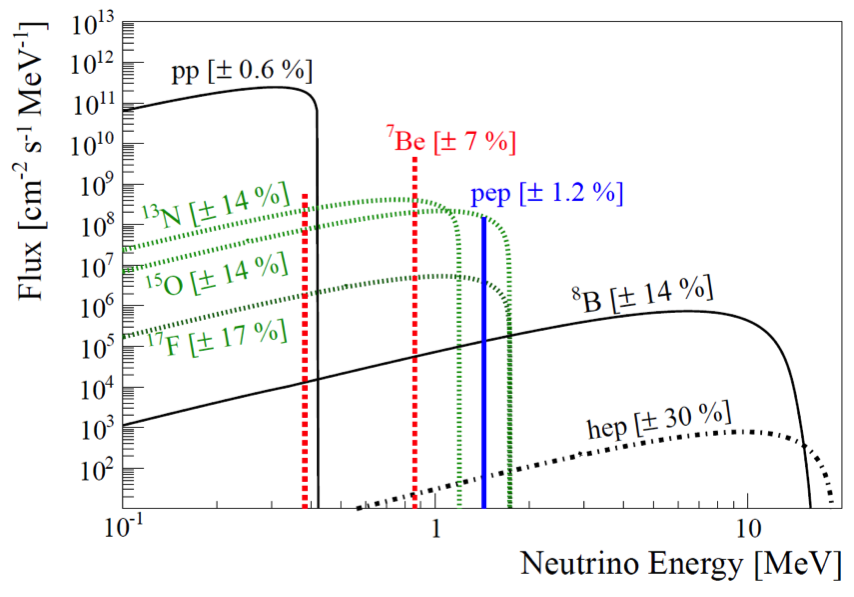
\includegraphics[width=0.7\textwidth]{figures/ch2-Theory/nu_spectrum.png}
     \caption[Solar neutrino spectrum]{Solar neutrino spectrum \cite{Borexino:2014lrx}}
        \label{fig:Solar-Neutrino-Spectrum}
\end{figure}

The earliest solar neutrino experiment, which was based in the Homestake Mine in South Dakota, used a radio-chemical method to measure the solar neutrino flux \cite{Lande:2003ex}. The detector consisted of a 615 tons massive tank of $C_2Cl_4$. The electron neutrinos interacted with the $Cl$ nuclei through inverse $\beta$-decay, producing radioactive $^{37}Ar$ nuclei which could then be counted through their decay products. The observed rate of interactions was $0.48\pm0.04 \ \nu/\text{day}$ which represented a significant deficit compared to the expected $1.7 \ \nu/\text{day}$. This anomaly became known as the solar neutrino problem and was later reproduced by other radio-chemical experiments like GALLEX \cite{GNO:2005bds} and SAGE \cite{SAGE:2002fps}. These experiments used Gallium as a target, making the low energy pp-cycle neutrinos accessible, whereas the Homestake detector was only sensitive to higher energy $\nu_e$'s from Boron decay.

The 50k ton Super-Kamiokande water Cerenkov experiment provided additional proof of the solar neutrino deficit phenomenon \cite{Super-Kamiokande:2001ljr}. The detector consists of a large vessel containing water surrounded by photo-multipliers capable of detecting Cerenkov radiation from relativistic charged particles. Solar neutrinos were detected through elastic $\nu_e \rightarrow \nu_e$ processes. The final-state electrons produced Cerenkov radiation that could be identified as a ring of hits on the sides of the detector. The number of photons gave a measure of the neutrino energy, while the orientation of the ring provided information on the direction of the particle. 

The angular distribution of the exiting electrons is isotropic with the centre of mass frame with respect of the incoming neutrino. Since the center of mass frame is boosted in the laboratory frame, the scattering electron follows roughly the direction of the $\nu_e$. Consequently, the directional correlation with the Sun is maintained, allowing the Super-Kamiokande experiment to provide clear evidence of a flux of $\nu_e$ from the Sun. This measurement confirmed the solar anomaly from the radio-chemical experiment, as the flux of electron neutrinos was measured to be half than expected.

\begin{figure}[t]
    \centering
    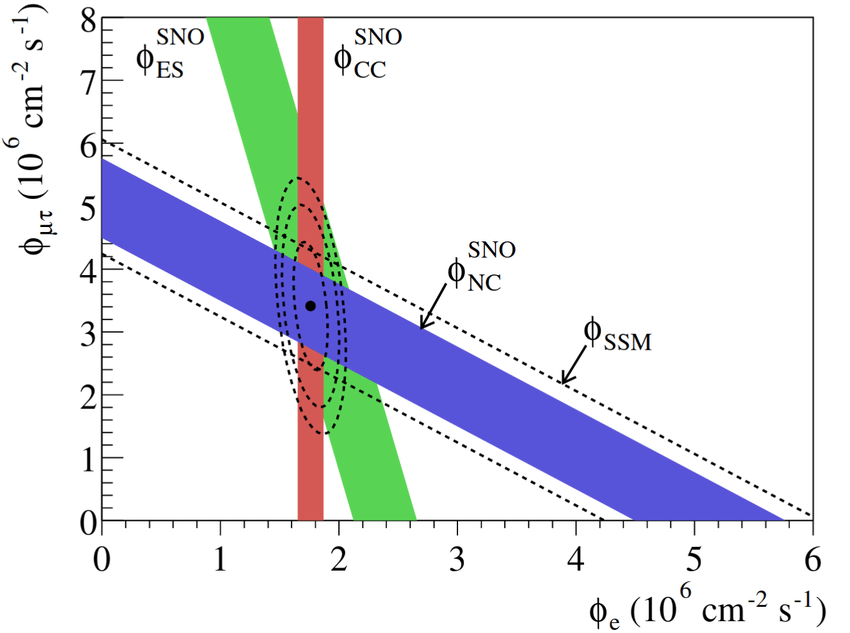
\includegraphics[width=0.7\linewidth]{figures/ch2-Theory/SNO.png}
    \caption[Evidence of solar neutrino oscillations from the SNO experiment]{Flux of $8B$ solar neutrinos which are $\mu$ or $\tau$ flavor vs flux of electron neutrinos deduced from the three neutrino reactions in SNO. The diagonal bands show the total 8B flux as predicted by the standard solar model (SSM) (dashed lines) and that measured with the NC reaction in SNO (solid band). The intercepts of these bands with the axes represent the $\pm 1 \sigma$ errors. \cite{SNO:2002tuh}}
    \label{fig:SNO}
\end{figure}

While the Super-Kamiokande experiment provided clear evidence for a deficit of solar neutrinos coming from the Sun, it gave no information regarding other neutrino species. The Sudbury Neutrino Observatory (SNO) was designed to measure both the $\nu_e$ flux and the total neutrino flux \cite{SNO:2002tuh}. SNO was a Cerenkov detector consisting of a vessel containing 1000 tons of heavy water and 9600 PMTs. The use of heavy water was motivated by the low binding energy of deuteron, which gave access to nuclear CC interactions, something that is not possible in standard water and that was unavailable to the Super-Kamiokande experiment. The CC channel $\nu_e+\text{D}\rightarrow e+ \text{p}+ \text{p}$ where the deuteron nucleon is broken up is only sensitive to the electron neutrino flux, making it possible to isolate it from the other flavours:
\begin{equation}
    \text{CC rate}\propto \phi(\nu_e) .
\end{equation}
The NC channel with consequent break-up of the deuteron nucleus $\nu_l+\text{D}->p+n$ was instead sensitive to the flux of all neutrino flavours. The neutron in the final state could be detected by measuring the electro-magnetic shower produced by the de-exitation photon ejected by a capturing hydrogen nucleus through the reaction: $\text{n}+^2_1\text{H} \rightarrow ^3_1\text{H}+\gamma$. The NC process is sensitive to the total neutrino flux:
\begin{equation}
    \text{NC rate}\propto \phi(\nu_e)+\phi(\nu_\mu)+\phi(\nu_\tau) .
\end{equation}
Neutrinos can also interact with atomic electrons through electronic scattering (ES). While for $\nu_e$ this process is available both through CC and NC interactions, it is only possible for $\nu_\mu$ and $\nu_\tau$ through NC interactions. The channel is thus sensitive to all neutrino fluxes but to differing degrees:
\begin{equation}
    \text{ES rate}\propto\phi(\nu_e)+0.154\left[\phi(\nu_\mu)+\phi(\nu_\tau)\right] .
\end{equation}
Since the electrons from ES maintain the directional information of the original neutrino, these interactions could be separated from the CC sample. Using all three processes SNO was capable of providing constraints on and separate the $\nu_e$ and $\nu_\mu+\nu_\tau$ fluxes obtaining the overall results:
\begin{equation}
    \begin{aligned}
        \phi(\nu_e)&=(1.76\pm0.10)\times 10^{-6} \text{cm}^{-2}\text{s}^-1 , \\
        \phi(\nu_\mu)+\phi(\nu_\tau)&=(3.41\pm0.63)\times 10^{-6} \text{cm}^{-2}\text{s}^-1 .
    \end{aligned}
\end{equation}
The SNO flux constraints are shown in Fig. The total neutrino flux was measured to be consistent with the expected $\nu_e$ flux coming from the Sun:
\begin{equation}
    \phi(\nu_e)_\text{exp} = (5.1\pm0.9)\times10^{-6}\text{cm}^{-2}\text{s}^-1 .
\end{equation}
The SNO data demonstrated that while the total flux of neutrinos coming from the Sun was consistent with expectation, about a third of it consisted of $\nu_\mu$ and $\nu_\tau$ neutrinos rather than $\nu_e$. Since only electron neutrinos can be produced in fusion reactions in the Sun, the SNO experiment was the first to give clear evidence of neutrino flavour oscillation transformation over large distances. This result initiated a new season in neutrino physics focused on the study of neutrino flavour oscillations. The SNO observations have since been confirmed by a variety of experiments using different neutrino sources and detection techniques and the phenomenon is still heavily under study today. 


%Using this technique the detector was sensitive to solar neutrinos with energies down to about 5 MeV, making the pp-cycle $\nu_e$ inaccessible.  

%%%Write paragraph with the history of the discovery of neutrino oscillations taking first few paragraphs from the modern particle physics cambridge book (probably about 1/2 pages worth) summary of chapter 13.2

\section{Theory of neutrino Oscillations}
\label{Sec:OscillationTheory}
The stationary states of the free-particle Hamiltonian are the mass eigenstates of the particle and they satisfy the equation:
\begin{equation}
\label{eq:Schroedinger1}
    \Hat{H}\psi = i\frac{\partial\psi}{\partial t} =E\psi .
\end{equation}
The time evolution of the mass eigenstates takes the form:
\begin{equation}
    \psi(\mathbf{x},t)=\phi(\mathbf{x})e^{-iEt} .
\end{equation}
The neutrinos have three mass eigenstates $\nu_1$, $\nu_2$ and $\nu_3$. In weak interactions however, neutrinos are produced as their weak eigenstates $\nu_e$, $\nu_\mu$ or $\nu_\tau$ alongside their respective flavour of charged lepton (see Eq. \ref{eq:weakeigenstates}). The neutrino mass eigenstates do not correspond to the weak eigenstates. Each neutrino flavour has to be described as a coherent linear super-position of the $\nu_1$, $\nu_2$ and $\nu_3$ states. The relationship between the weak and mass eigenstates can be described using the Pontecorvo-Maki-Nakagawa-Sakata (PMNS) unitary mixing matrix $U_\text{PMNS}$ as \cite{Thomson_2013}:
\begin{equation}
\label{eq:PMNS1}
    \begin{pmatrix}
        \nu_e \\ \nu_\mu \\ \nu_\tau
    \end{pmatrix}
    = U_\text{PMNS}
    \begin{pmatrix}
        \nu_1 \\ \nu_2 \\ \nu_3
    \end{pmatrix}   
    =
    \begin{pmatrix}
        U_{e1} & U_{e2} & U_{e3} \\
        U_{\mu 1} & U_{\mu 2} & U_{\mu 3} \\
        U_{\tau 1} & U_{\tau 2} & U_{\tau 3} 
    \end{pmatrix}
    \begin{pmatrix}
        \nu_1 \\ \nu_2 \\ \nu_3
    \end{pmatrix} ,
\end{equation}
with the unitarity condition being: 
\begin{equation}
    \begin{pmatrix}
        U_{e1} & U_{e2} & U_{e3} \\
        U_{\mu 1} & U_{\mu 2} & U_{\mu 3} \\
        U_{\tau 1} & U_{\tau 2} & U_{\tau 3} 
    \end{pmatrix}
    \begin{pmatrix}
        U_{e1}^* & U_{\mu1}^* & U_{\tau1}^* \\
        U_{e2}^* & U_{\mu2}^* & U_{\tau2}^* \\
        U_{e3}^* & U_{\mu3}^* & U_{\tau3}^* 
    \end{pmatrix}
    =
    \begin{pmatrix}
        1 & 0 & 0 \\
        0 & 1 & 0 \\
        0 & 0 & 1
    \end{pmatrix} .
\end{equation}
If we consider an electron neutrino produced in a weak interaction at the vertex $W^+ \rightarrow e^+\nu$, its wave function will be a linear combination of the three mass eigenstates defined by their relative weak interaction couplings $U_{ei}^*$ as:
\begin{equation}
    \left| \psi\right\rangle = U^*_{e1}\left| \nu_1\right\rangle + U^*_{e2}\left| \nu_2\right\rangle + U^*_{e3}\left| \nu_3\right\rangle .
\end{equation}

The neutrino state then propagates as a linear combination of the mass eigenstates until it interacts, collapsing into a weak eigenstate and producing a specific lepton flavour. If the three neutrino masses are not the same, phase differences are generated between the different wave-function components, giving rise to the phenomenon of neutrino oscillations. 


\subsection{Two flavour scenario}
\label{Sec:2flavour}
%From Cambrige book chapter 13.4 https://ereader.cambridge.org/wr/viewer.html?skipLastRead=true#book/1f090751-c7b7-4e1e-bca5-40536f8e8a53/body20
While neutrinos in the standard model have three flavours and mass eigenstates, flavour oscillations can be more easily derived in a two-flavour scenario, without losing many of the key features of the phenomenon. Let's consider the weak eigenstates $\nu_e$ and $\nu_\mu$ which are linear superpositions of the mass eigenstates $\nu_1$ and $\nu_2$. The weak eigenstates are related to the mass eigenstates by a unitary $2\times 2$ matrix which can be written as a function of a single mixing angle $\theta$:
\begin{equation}
    \begin{pmatrix}
        \nu_e \\ \nu_\mu
    \end{pmatrix}
    =
    \begin{pmatrix}
        \cos \theta & \sin \theta \\
        -\sin\theta & cos \theta
    \end{pmatrix}
    \begin{pmatrix}
        \nu_1 \\ \nu_2
    \end{pmatrix} .
\end{equation}

Let's suppose that an electron neutrino $\nu_e$ is produced trough a weak interaction process. The propagation of its wave-function through space can be written according to the time dependence of the mass eigenstates:
\begin{equation}
\label{eq:xttravel}
    \left| \psi(L,T)\right\rangle = \cos\theta \left|\nu_1\right\rangle e^{-\phi_1}+ \sin\theta \left|\nu_1\right\rangle e^{-\phi_2} ,
\end{equation}
where the phases of the two eigenstates can be written as: 
\begin{equation}
    \phi_i = p_i\cdot x = E_i-\text{p}_i L ,
\end{equation}
with $p_i$ and $x$ being the 4-momenta and 4-positions of the mass eigenstates, $E_i$ and $\text{p}_i$  their energies and total momenta, and $T$ and $L$ the time passed and distance travelled since production.  By rewriting the mass eigenstates as a linear combination of weak eigenstates Eq. \ref{eq:xttravel} can be re-written as:
\begin{equation}
\label{eq:xtflavourev}
    \begin{aligned}
        \left| \psi(L,T)\right\rangle & = e^{-i\phi_1} [ (\cos^2\theta+e^{i\Delta \phi_{12}}\sin^2\theta) \left|\nu_e\right\rangle 
        - (1-e^{-i\Delta\phi_{12}})\cos\theta\sin\theta \left|\nu_\mu\right\rangle] \\
        &=c_e\left|\nu_e\right\rangle + c_\mu\left|\nu_\mu\right\rangle ,
    \end{aligned}
\end{equation}
where $\Delta \phi_{12} = \phi_1 - \phi_2$ is the difference between the phases. If $\Delta\phi_{12}=0$ the neutrino remains a pure electron neutrino state, while if $\Delta\phi_{12}\neq0$ a muon neutrino component is introduced in the wave function. The probability that the neutrino which was produced as a $\nu_e$ will interact as a $\nu_\mu$ is $P(\nu_e \rightarrow \nu_\mu)=c_\mu c_\mu^*$.  Conversely the probability of the particle maintaining the initial flavour, sometimes referred to as survival probability, is simply $P(\nu_e\rightarrow \nu_e)=1-P(\nu_e \rightarrow \nu_\mu)$ . From Eq. \ref{eq:xtflavourev} $P(\nu_e \rightarrow \nu_\mu)$ can be written as:
\begin{equation}
\label{eq:2fOscprob1}
    P(\nu_e\rightarrow\nu_\mu) = \sin^2(2\theta)\sin^2\left(\frac{\Delta\phi_{12}}{2}\right) .
\end{equation}
The probability then depends on the mixing angle $\theta$ and the difference between the phases of the neutrino mass eigenstates $\Delta\phi_{12}$. The phase difference can be re-written as a function of the neutrino masses. If we assume that the momenta of the two mass eigenstates are equal $\text{p}_1 = \text{p}_2 = \text{p}$ the phase difference becomes:
\begin{equation}
    \Delta\phi_{12}=(E_1-E_2)T=\left[\text{p}\left(1+\frac{m_1^2}{\text{p}^2}\right)^{1/2}-\text{p}\left(1+\frac{m_2^2}{\text{p}^2}\right)^{1/2}\right] .
\end{equation}

\begin{figure}[t]
     \centering
     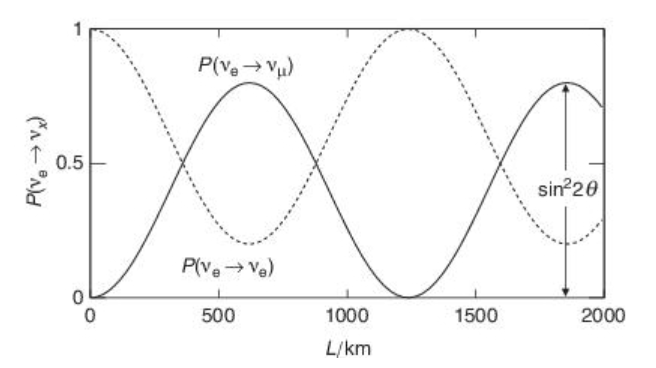
\includegraphics[width=0.7\textwidth]{figures/ch2-Theory/Oscillation2F.png}
     \caption[Two-flavour oscillation probability]{The two-flavour oscillation probability $P(\nu_e \rightarrow \nu_\mu)$ and the survival probability $P(\nu_e \rightarrow \nu_e)$ plotted as function of $L$ for $E_\nu= 1 \ \text{GeV}$, $\Delta m^2=0.0002 \ \text{eV}^2$ and $\sin^2(2\theta)=0.8$ \cite{Thomson_2013}.}
        \label{fig:Oscillation2F}
\end{figure}
Under the assumption that neutrinos are very light and thus $m\ll E$ one can use the first order approximation $\sqrt{1+x^2}\approx1+x^2/2$ and re-write the phase difference as:
\begin{equation}
\label{eq:deltaphi12}
    \Delta \phi_{12} \approx \frac{m_1^2-m_2^2}{2\text{p}}L .
\end{equation}
Eq. \ref{eq:2fOscprob1} can finally be re-written as:
\begin{equation}        P(\nu_e\rightarrow\nu_\mu)=\sin^2(2\theta)\sin^2\left(\frac{\Delta m^2 L}{4E_\nu}\right) ,       
\end{equation}
where $p=E_\nu$ and $\Delta m^2 = m_1^2-m_2^2$. An illustrative example of the evolution of the oscillation probabilities as a function of distance is shown in Fig \ref{fig:Oscillation2F}. For small values of $\Delta m^2$, neutrino flavour oscillations can only develop over very large distances. The amplitude of the oscillation is determined by $\sin^2(2\theta)$, with mixing being maximal when $\sin^2(2\theta)=1$ i.e. when $(\theta = \pi/4)$.

\subsection{Three flavour scenario}
%Write down PMNS matrix from Kang's thesis and write down the oscillation probability from the DUNE chapter.
In the three flavour scenario the PMNS mixing matrix, which describes the relationship between the flavour and mass eigenstates contains three mixing angles $\theta_{12}$, $\theta_{23}$ and $\theta_{13}$ and one complex phase $\delta_\text{CP}$.
\begin{equation}
\begin{aligned}
U_{\text{PMNS}} &= 
\begin{pmatrix}
1 & 0 & 0 \\
0 & c_{23} & s_{23} \\
0 & -s_{23} & c_{23}
\end{pmatrix}
\begin{pmatrix}
c_{13} & 0 & s_{13} e^{-i\delta_{CP}} \\
0 & 1 & 0 \\
-s_{13} e^{i\delta_{CP}} & 0 & c_{13}
\end{pmatrix}
\begin{pmatrix}
c_{12} & s_{12} & 0 \\
-s_{12} & c_{12} & 0 \\
0 & 0 & 1
\end{pmatrix} \\
&=
\begin{pmatrix}
c_{12} c_{13} & s_{12} c_{13} & s_{13} e^{-i\delta_{CP}} \\
-s_{12} c_{23} - c_{12} s_{23} s_{13} e^{i\delta_{CP}} & c_{12} c_{23} - s_{12} s_{23} s_{13} e^{i\delta_{CP}} & s_{23} c_{13} \\
s_{12} s_{23} - c_{12} c_{23} s_{13} e^{i\delta_{CP}} & -c_{12} s_{23} - s_{12} c_{23} s_{13} e^{i\delta_{CP}} & c_{23} c_{13} ,
\end{pmatrix}
\end{aligned}
\end{equation}

where $c_{ij}$ and $s_{ij}$ stand for $\cos\theta_{ij}$ and $\sin\theta_{ij}$ respectively. The derivation of the neutrino oscillation probability can be done following a procedure that is fully analogous to what was described in the 2-flavour scenario. If we consider an electron neutrino produced in a weak interaction, the time evolution of its wave-function can be described as the superposition of the time evolution of the mass eigenstates:
\begin{equation}
    \left|\psi(x,t)\right\rangle = U_{e1}^*\left|\nu_1\right\rangle e^{-i\phi_1}+
    U_{e2}^*\left|\nu_2\right\rangle e^{-i\phi_2}+
    U_{e3}^*\left|\nu_1\right\rangle e^{-i\phi_3} .
\end{equation}
We can then re-write the mass eigenstates as a linear superposition of the three weak eigenstates. By doing this and grouping the terms for each weak eigenstate we obtain:
\begin{equation}
    \begin{aligned}
        \left|\psi(x,t)\right\rangle =&
        (U^*_{e1}U_{e1}e^{-i\phi_1}+
         U^*_{e2}U_{e2}e^{-i\phi_2}+
         U^*_{e3}U_{e3}e^{-i\phi_3})
         \left|\nu_e\right\rangle
        + \\ &
        (U^*_{e1}U_{\mu1}e^{-i\phi_1}+
         U^*_{e2}U_{\mu2}e^{-i\phi_2}+
         U^*_{e3}U_{\mu3}e^{-i\phi_3})
         \left|\nu_\mu\right\rangle
        + \\ &
        (U^*_{e1}U_{\tau1}e^{-i\phi_1}+
         U^*_{e2}U_{\tau2}e^{-i\phi_2}+
         U^*_{e3}U_{\tau3}e^{-i\phi_3})
         \left|\nu_\tau\right\rangle =
        \\ &
        =c_e \left|\nu_e\right\rangle+
        c_\mu\left|\nu_\mu\right\rangle+
        c_\tau\left|\nu_\tau\right\rangle .
    \end{aligned}
\end{equation}
The oscillation probability can be obtained similarly to the 2-flavour scenario and is defined in terms of the flavours of the charged leptons produced in the weak interactions and the relevant PMNS matrix elements:
\begin{equation}
\label{eq:3fprob}
    P(\nu_e\rightarrow\nu_\mu) = c_\mu c_\mu^* = |U_{e1}^*U_{\mu1}e^{-i\phi_1}+U_{e2}^*U_{\mu2}e^{-i\phi_2}+U_{e2}^*U_{\mu2}e^{-i\phi_2}|^2 .
\end{equation}
If the phases were all the same then the unitarity condition $U_{e1}^*U_{\mu1}+U_{e2}^*U_{\mu2}+U_{e3}^*U_{\mu3}=0$ would imply that the oscillation probability is null. Neutrino oscillations can only occur if neutrinos have masses and these masses are different. Using the approximation outlined Eq. \ref{eq:deltaphi12} and generalizing the results of Eq. \ref{eq:3fprob} the oscillation probability between two generic flavour eigenstates $P(\nu_\alpha\rightarrow\nu_\beta)$ can be written as:
\begin{equation}
\begin{aligned}   
\label{eq:3fosc_proper}
    P(\nu_\alpha \rightarrow \nu_\beta) = \delta_{\alpha\beta} &
    -4 \sum_{j>k}\Re\left[U_{\alpha j}^*U_{\beta j}U_{\alpha k}U_{\beta k}^*\right]\sin^2\left(\frac{\Delta m^2_{jk}L}{4E_\nu}\right) \\
    & +2 \sum_{j>k}\Im\left[U_{\alpha j}^*U_{\beta j}U_{\alpha k}U_{\beta k}^*\right]\sin\left(\frac{\Delta m^2_{jk}L}{2E_\nu}\right) .
\end{aligned}
\end{equation}
It's important to note that the second sum in the expression is non-zero only if the imaginary phase $\delta_\text{CP}$ is non-zero. Measuring neutrino oscillation probabilities and the parameters that govern it, is a major topic in modern particle physics. A summary of the most precise measurements currently available is presented in Tab. \ref{tab:OscProps}. In modern experiments particular attention is currently given to the $\delta_\text{CP}$ and the neutrino mass splittings $\Delta m_{ij}^2$ and their sign, for which the sensitivity is much less definitive than for the mixing angles.

\begin{table}
    \centering
    \begin{tabular}{||c|c|c||}
    \hline 
    Parameter & Measurement & Mass Order \\ 
    \hline \hline
    $\sin^2 \theta_{12}$ & 
    $0.307 \pm 0.013$ & \\
    \hline
    $\sin^2 \theta_{23}$ & 
    $0.539 \pm 0.022$ &  Inverted\\
    \hline
    $\sin^2 \theta_{23}$ & 
    $0.546 \pm 0.021$ &  Normal\\
    \hline
    $\sin^2 \theta_{13}$ & 
    $(2.20 \pm 0.07)\times 10^{-2}$ &  Normal\\
    \hline
    $\Delta m_{21}^2$ & 
    $(7.53 \pm 0.18)\times 10^{-5} \ \text{eV}^2$ &  \\
    \hline
    $\Delta m_{32}^2$ & 
    $(-2.536 \pm 0.034)\times 10^{-3} \ \text{eV}^2$ &  Inverted\\
    \hline
    $\Delta m_{32}^2$ & 
    $(2.456 \pm 0.033)\times 10^{-3} \ \text{eV}^2$ &  Normal\\
    \hline
    $\delta_\text{CP}$ & 
    $1.36^{+0.20}_{-0.16}\pi \ \text{rad}$ &  \\
    \hline 
    \end{tabular}
    \caption{Summary of best currently available experimental results for neutrino oscillation parameters \cite{ParticleDataGroup:2022pth}. When the results are dependent on neutrino mass hierarchy (see Sec. \ref{Sec:Neutrinomasses}), the ordering is specified.}
    \label{tab:OscProps}
\end{table}
\subsection{Charge-Parity Symmetry Violation}
Three fundamental discrete symmetries exist in particle physics: charge conjugation $\Hat{C}$ turns a particle into an anti-particle; parity $\Hat{P}$ reverses the spatial component of the wave-function; time $\Hat{T}$ reverses the time component of the interaction. It has been demonstrated experimentally that the weak interaction violates both $\Hat{P}$ and $\Hat{C}$ symmetry \cite{Boyde2005}. Let's consider for example the pion decay $\pi \rightarrow \mu^- + \Bar{\nu}_\mu$ illustrated in Fig. \ref{fig:piondecay}. The parity operator $\Hat{P}$ inverts the direction of the particle but not the spin, resulting in a left-handed anti-neutrino, which is not allowed. Charge conjugation $\Hat{C}$ transforms a particle into its own anti-particle, resulting in the decay $\pi^+ \rightarrow \mu^+ + \nu_\mu$ where the neutrino is right-handed, which is also not allowed. The application of $\Hat{C}\Hat{P}$ changes left-handed particles into right-handed anti-particles and the resulting decay can happen. 

The conservation of the CP symmetry implies that the probability of a particular interaction happening is identical to the probability of the CP transformed interaction occurring. It is known that that CP conservation is not respected in the quark sector \cite{Bona:2024bue}. In the context of neutrino oscillation CP invariance would imply:
\begin{equation}
    P(\nu_\alpha \rightarrow \nu_\beta) = P(\Bar{\nu}_\beta \rightarrow \Bar{\nu}_\alpha) .
\end{equation}
The unitarity conditions of the PMNS matrix however allow for an imaginary CP-violating phase $\delta_\text{CP}$ to exist. If $\delta_\text{CP}\neq 0$ the imaginary component of the oscillation probability in Eq. \ref{eq:3fosc_proper} is also non zero and changes sign when the $\Hat{C}\Hat{P}$ operator is applied, breaking the symmetry and resulting in $    P(\nu_\alpha \rightarrow \nu_\beta) \neq P(\Bar{\nu}_\beta \rightarrow \Bar{\nu}_\alpha)$.
\begin{figure}
    \centering
    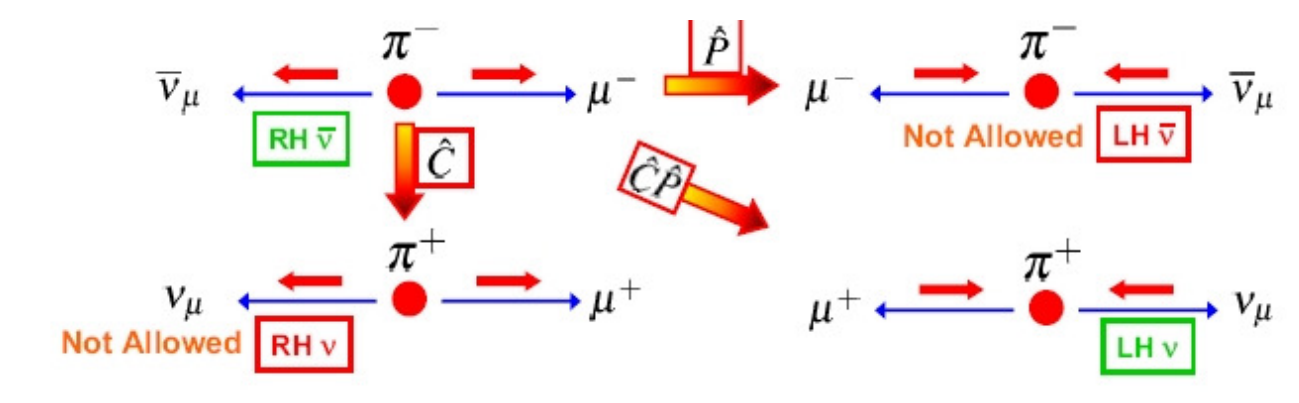
\includegraphics[width=0.9\linewidth]{figures//ch2-Theory/piondecay.png}
    \caption[$\Hat{C}$ and $\Hat{P}$ violation in pion weak decay]{$\Hat{C}$ and $\Hat{P}$ violation in pion weak decay. The blue arrows are the particle, and the red arrows show the spin vectors of each particle \cite{Boyde2005}.}
    \label{fig:piondecay}
\end{figure}
The CP-asymmetry can be quantified as the difference between the two probabilities:
\begin{equation}
\begin{aligned}
    \mathcal{A}^\text{CP}_{\alpha\beta} &= P(\nu_\alpha \rightarrow \nu_\beta)-P(\Bar{\nu}_\beta \rightarrow \Bar{\nu}_\alpha) = \\
    &=4 \sum_{j>k}\Im\left[U_{\alpha j}^*U_{\beta j}U_{\alpha k}U_{\beta k}^*\right]\sin\left(\frac{\Delta m^2_{jk}L}{2E_\nu}\right) ,
\end{aligned}
\end{equation}
which is often written in terms of the Jarslog invariant $J_\text{CP}$ as:
\begin{equation}
    \begin{aligned}
    \mathcal{A}^\text{CP}_{\alpha\beta}&=16\sin\left(\frac{\Delta m^2_{21}L}{4E_\nu}\right) \sin\left(\frac{\Delta m^2_{32}L}{4E_\nu}\right) \sin\left(\frac{\Delta m^2_{31}L}{4E_\nu}\right) J_\text{CP} \sum_{\gamma}\varepsilon_{\alpha\beta\gamma}\\
    \text{with } & \Im\left[U^*_{\alpha j}U_{\beta j}U_{\alpha k}U^*_{\beta k}\right] = J_{\text{CP}} \sum_{\gamma,l} . %\varepsilon_{\alpha \beta \gamma} \varepsilon_{jkl}
    \end{aligned}
\end{equation}

Current measurements of $\delta_\text{CP}$ lack the precision necessary to definitively determine whether the neutrino oscillation CP violation exists. The determination of the CP violating phase is thus a major topic of research in modern neutrino physics.

%Combination of Kang's thesis https://ora.ox.ac.uk/objects/uuid:b2efbb9b-1ccc-4aa6-9081-8a9ca9595b2b/files/d05741s28c and my master thesis https://amslaurea.unibo.it/20447/1/TesiFB.pdf
%Used this warwick.ac.uk/fac/sci/physics/staff/academic/boyd/stuff/neutrinolectures/lec_oscillations.pdf in the first bit and then my thesis 
\subsection{Neutrino masses and mass hierarchy}
\label{Sec:Neutrinomasses}

%From Modern particle physics textbook + my thesis
Neutrino oscillations depend on the differences of the squared neutrino masses, not the masses themselves. It is thus not possible to use neutrino oscillations to constrain the overall neutrino mass scale. Other strategies can however be used, even though only upper limits have been achieved so far. Constraints on the mass of the lightest neutrino can be obtained by measuring the end point of the electron energy distribution in the nuclear $\beta$-decay of tritium. To date the most sensitive measurements obtained come from the KATRIN experiment, which set the limit at $m_\nu<1.1 \ \text{eV}$ at 90\% confidence level \cite{KATRIN:2019yun}. Tighter model dependent constraints on the sum of all neutrino masses can be obtained from cosmological measurements. The density of relic neutrinos from the Big Bang is large and can impact the evolution of the universe. Recent cosmological measurements on the large scale structure of the universe set this limit at $\sum_i m_{i}\leq0.12 \ \text{eV}$ \cite{Gariazzo:2024beg}.

\begin{figure}
    \centering
    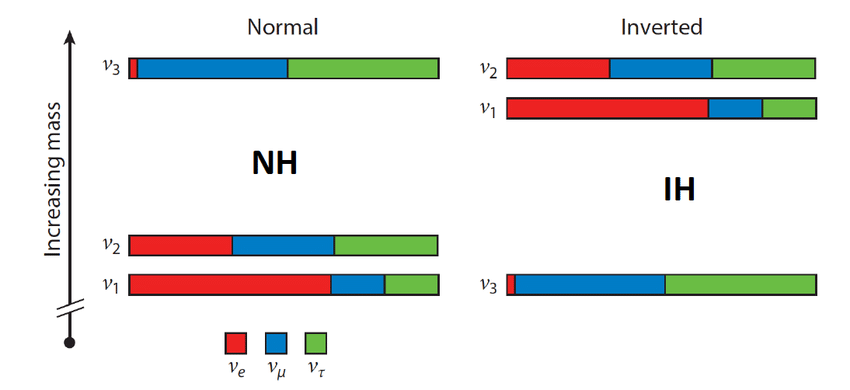
\includegraphics[width=0.75\linewidth]{figures//ch2-Theory/MassOrder.png}
    \caption[Illustration of the neutrino mass ordering.]{Illustration of the neutrino mass ordering for the two hypotheses, Normal Hierarchy (NH) and Inverted Hierarchy (IH). The flavour sharing due to the mixing is also drawn for each mass eigenstate.  
 \cite{Stanco:2016usn}}
    \label{fig:MassOrdering}
\end{figure}

While oscillation experiments cannot distinguish between the individual neutrino masses, they can provide measurements of the squared neutrino mass differences (see Tab. \ref{tab:OscProps}). An important aspect of modern neutrino oscillation physics is the determination of the neutrino mass hierarchy (MH) , which refers to the ordering of the three neutrino mass eigenstates. Regardless of the absolute mass scale of the lightest neutrino, two possible hierarchies exist, as shown in Fig. \ref{fig:MassOrdering}. The scenario in which the lightest mass eigenstate is $\nu_1$, followed in order by $\nu_2$ and $\nu_3$ is referred to as the normal hierarchy (NH), while the alternative scenario in which $\nu_3$ is the lightest, followed by $\nu_1$ and $\nu_2$ is referred to as the inverted hierarchy (IH).  
\subsection{Matter effects}
\label{Sec:MSW}
%My master thesis https://amslaurea.unibo.it/20447/1/TesiFB.pdf

When neutrinos travel through matter they interact with electrons and nuclei in the medium. These interactions effectively modify the oscillation probabilities in a way that depends on the flavours of the neutrinos. This is due to the fact that while $\nu_e$'s take part in both NC and CC interactions with electrons, $\nu_\mu$'s and $\nu_\tau$'s only participate in NC interactions. This matter effect is known as Mikhaev, Smirnov and Wolfenstein (MSW) effect \cite{Mikheyev:1985zog,Smirnov:2003da,Wolfenstein:1977ue}. 

The MSW effect can be easily described in the 2-flavour scenario \cite{Ricciardi2003}. The time evolution Schroedinger equation in eq. \ref{eq:Schroedinger1} can be re-written using the 2-flavour mixing matrix as:
\begin{equation}
    \Hat{H}
    \begin{pmatrix}
        \nu_e \\ \nu_\mu
    \end{pmatrix} = 
    i\frac{d}{dt}
    \begin{pmatrix}
    \nu_e \\ \nu_\mu
    \end{pmatrix}
    \text{  where  }
    \Hat{H}=
    \left(\frac{\Delta m^2}{4E_\nu}\right) 
    \begin{pmatrix}
        -\cos2\theta & \sin2\theta \\
        \sin{2\theta} & \cos{2\theta}
    \end{pmatrix} .
\end{equation}
The enhanced interaction probability experienced by $\nu_e$'s can be effectively described by an extra potential $V_e = \pm \sqrt{2} G_F N_e$, where $N_e$ is the electron density, $G_F$ is the Fermi constant and the positive (negative) sign applies to electron neutrinos (anti-neutrinos). Using this potential we can construct an effective Hamiltonian $\Hat{H}_M$ which describes the propagation of neutrinos in matter:
\begin{equation}
    \Hat{H}_M = \Hat{H}+
    \begin{pmatrix}
        V_e & 0\\
        0   & 0
    \end{pmatrix}
    =     \left(\frac{\Delta m^2}{4E_\nu}\right) 
    \begin{pmatrix}
        -\cos2\theta & \sin2\theta \\
        \sin{2\theta} & \cos{2\theta}
    \end{pmatrix} +
        \begin{pmatrix}
        V_e & 0\\
        0   & 0
    \end{pmatrix} .
\end{equation}
In the simple case where the matter density is constant, the effective Hamiltonian $\Hat{H}_M$ can be re-diagonalised to obtain a new mixing matrix:
\begin{equation}
    \Hat{H}_M=
    \left(\frac{\Delta m^2_M}{4E_\nu}\right) 
    \begin{pmatrix}
        -\cos2\theta_M & \sin2\theta_M \\
        \sin{2\theta}_M & \cos{2\theta_M}
    \end{pmatrix} . 
\end{equation}
where $\theta_M$ and $\Delta m_M^2$ are the new effective oscillation parameters. They can be written as:
\begin{equation}
    \begin{aligned}
        \Delta m^2_M & = M \Delta m^2 ,\\
        \sin 2 \theta_M & = \frac{\sin 2 \theta}{M} , 
    \end{aligned}
\end{equation}
with the coefficient $M$ being 
\begin{equation}
    M = \sqrt{\left(\cos 2\theta - \Hat{A}\right)^2 + \sin^2 2 \theta} ,
\end{equation}
and 
\begin{equation}
    \Hat{A} = \pm \frac{2\sqrt{2}G_F N_e E_\nu}{\Delta m^2} .
\end{equation}
The sign of $\Hat{A}$ is positive for neutrinos and negative for anti-neutrinos. Using the new effective parameters the oscillation probability in matter becomes
\begin{equation}
    P(\nu_e \rightarrow \nu_\mu) = \sin^2 2 \theta_M \sin^2 \left(\frac{\Delta m^2_M L}{4 E_\nu}\right) .
\end{equation}
The MSW effect modifies neutrino oscillation probabilities in some crucial ways. Due to the $\pm$ sign in front of $\Hat{A}$ a difference in behaviour between neutrinos and anti-neutrinos is introduced without CP violation. Additionally a resonant condition exists for which the oscillation probability is significantly enhanced with respect to the one in vacuum, which is when $\Hat{A}= \cos 2 \theta$. The resonant condition can be met only if $\Hat{A}>0$, which in turn depends on the sign of the squared mass difference $\Delta m^2$. This fact can be exploited to study the neutrino mass ordering. However, either long travel distances or high matter densities are necessary in order for the MSW effects to be appreciable. In the case where $\Delta m_M^2 L /4 E_\nu \ll 1$ the neutrino oscillation probabilities are indistinguishable from the ones in vacuum.


\section{Neutrino sources}
\label{Sec:NeutrinoSources}
The key principles that govern neutrino production in neutrino experiments have remained remarkably consistent since the early days of neutrino physics \cite{T2KNotes}. The following summary provided by Fred Reines in a review article in the 1960s \cite{Reines:1960we} is largely still valid today : 
\begin{itemize}
    \item Fission reactors are an optimal source of low energy $\Bar{\nu}_e$;
    \item A flux of $\nu_\mu$ and $\Bar{\nu}_\mu$ can be produced by allowing charged pions of the correct charge to decay in flight and then stopping the hadrons produced in the decay using a dense absorber;
    \item The Sun serves as a significant source of neutrinos, primarily produced through various nuclear fusion processes. However, the majority of these neutrinos are generated at low energies, making their detection challenging. The detectability of solar neutrinos largely depends on the presence of alternative fusion pathways, such as those involving boron-8 and beryllium-7, which produce higher-energy neutrinos;
    \item Cosmic rays interacting with the Earth's atmosphere generate a substantial flux of neutrinos as a result of pion decay;
    \item High-energy neutrinos produced by astrophysical objects can provide unique information that is not accessible through cosmic rays, which are deflected by the Galaxy’s magnetic field, or photons, which can be absorbed by dense matter;
\end{itemize}
 In this section we discuss the role of these sources in modern neutrino physics separating them into natural and artificial.
%Get from T2K guide https://t2k-experiment.org/neutrinos/
\subsection{Artificial neutrino sources}
\label{Sec:artificial}
The two main types of artificial neutrino sources are nuclear fission reactors, which produce low energy $\Bar{\nu}_e$ as a bi-product of the fission reaction chain, and proton accelerators, from which $\Bar{\nu}_\mu$ and $\nu_\mu$ fluxes can be obtained.

Fission reactors produce energy by breaking up heavy nuclei, typically U-235, using a flow of slow neutrons and maintaining a controlled chain reaction. As the ratio of neutrons to protons is higher for heavier nuclei, the fission products tend to be unstable and undergo a cascade of $\beta$-decays which in turn produce several $\Bar{\nu}_e$'s. Each fission reaction produces on average 6 neutrinos. Knowing the reactor's energy output, it is then possible to estimate the rate of electron anti-neutrino production. For neutrino experiments it is however not sufficient to know the rate of production. The energy spectrum of the neutrinos also needs to be determined, since both the interaction cross-sections in the detectors as well as the oscillation probabilities depend on it. Estimating this is much more complex, because a variety of different fissionable nuclei and fission fragments can be produced in the reaction, all of which have different decay spectra. 

Several techniques can be applied to estimate the energy of the fission neutrinos. The spectrum can be estimated from first principles using data collected from all past nuclear reactors on fission products and their decay spectra. This approach is, however, heavily model dependent. The spectrum of the neutrinos can also be inferred from the spectrum of the electrons, which are also produced in the $\beta$-decay and can be measured directly. This approach also requires some knowledge of the underlying $\beta$-decays but not as much as the previous method. While these techniques are well established and produce reliable estimates, the modelling of neutrino spectra is still a major source of systematic uncertainty. For this reason modern reactor neutrino oscillation experiments employ a near detector which measures the neutrinos close to the source and a far detector placed at a distance which maximizes the oscillation probability. This configuration allows to reduce to a minimum uncertainties on how the beam evolves with distance. Additionally, uncertainties related to the modelling of the reactor neutrino flux largely cancel out.

\begin{figure}
    \centering
    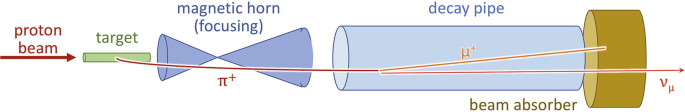
\includegraphics[width=\linewidth]{figures//ch2-Theory/NeutrinoBeam2.png}
    \caption[A schematic diagram of a typical neutrino beam production procedure.]{A schematic diagram of a typical neutrino beam production procedure. Both neutrino and anti-neutrino beams can be produced by switching modes of the focusing horns to select pions of the preferred charge \cite{Wurm2021}. }
    \label{fig:Neutrino beam}
\end{figure}

Neutrino beams can also be produced using an accelerated beam of protons. The protons are accelerated using a particle accelerator, typically a synchrotron; they can then be extracted from the accelerator and directed on to a target; finally they interact with the target producing many secondary particles among other particles. Magnetic focusing horns are then used to isolate pions of a specific charge and focus them into a beam. The beam is then directed into a long decay tunnel where positive pions decay into a $\mu^+$ and $\nu_\mu$ while negative pions decay into a $\mu^-$ and $\Bar{\nu}_\mu$.  The length of the tunnel is designed so that most pions decay, but not many muons do. While the typical pion lifetime is relatively short at $0.026 \ \mu \text{s}$, when time dilation is taken into consideration the average decay length, which determines the length of the decay tunnel, can be up to $\sim 100 \ \text{m}$ long. At the end of the decay tunnel a large mass of material (i.e. the beam dump) is placed so that all remaining particles are absorbed except for neutrinos. A schematic diagram of the production procedure is shown in Fig. \ref{fig:Neutrino beam}. 

The $\nu_\mu/\Bar{\nu}_\mu$ beams produced using this technique are very pure and only include a small irreducible contamination of $\nu_e$ generated from kaon decay. The modelling of the neutrino energy spectrum can be done from first principles and is significantly less challenging than for reactor beams. However, given the levels of precision required by contemporary accelerator experiments, all modern set-ups follow the Near/Far detector set-up outlined for the reactor experiments. Finally, it's important to note that the energy spectra in accelerator experiments tend to be very broad. They can however be significantly narrowed by using off-axis beams, at the cost of a reduced intensity. This technique was pioneered by the T2K experiment to generate a neutrino beam of well-defined energy \cite{T2K:2012qoq}.
\subsection{Natural neutrino sources}
As previously outlined in Sec. \ref{Sec:NuHistory} the discovery of neutrino oscillations was achieved, not with artificial sources, but using neutrinos naturally produced in the Sun. The Sun generates energy by fusing hydrogen to helium. Since an hydrogen nucleus is composed of a single proton, while helium contains two protons and two nucleons, the process involves the conversions of protons to neutrons and the emission of electron neutrinos. The main process through which this happens is the so-called pp chain, which produces low energy neutrinos as a bi-product. Other higher energy neutrinos are produced in rarer processes such as Be-7 and B-8 decays, which are part of the pp-II and pp-III side chains, or in the pep and hep chains which are even rarer. All these fusion processes contribute to the overall solar neutrino spectrum (see Fig. \ref{fig:Solar-Neutrino-Spectrum}). 

Massive quantities of neutrinos are produced in supernova explosions which mark the death of stars. Two types of supernova explosions exist. Type 1a supernovas are believed to originate in the destruction of white dwarf stars that have become too massive to support itself against gravity. These are used in cosmology because of their very consistent intrinsic brightness, but are not expected to produce many neutrinos. Core-collapse supernovae arise as end of life events for massive stars. 99\% of the energy released by these types of supernova comes in the form of neutrinos (see Sec. \ref{sec:SupernovaNeutrinos} for a more detailed discussion).

The Earth is constantly bombarded by cosmic rays, which are mostly composed by protons and a smaller percentage $\sim10-15\%$ of cosmic rays. When the protons interact with the Earth's atmosphere they produce pion showers which decay to muons and muon neutrinos in a way that is analogous to the production of neutrino beams in accelerator experiments. Muons either reach the Earth's surface or decay themselves producing some $\nu_\mu$ and $\nu_e$. If all muons decayed in flight we would expect a 2:1 ratio between muon and electron neutrinos, but since this is not the case the expected percentage of $\nu_\mu$ is increased. Early measurements of atmospheric neutrinos showed a significant deficit in the number of muon neutrinos when compared to expectations, giving rise to the so-called atmospheric neutrino anomaly. The Super-Kamiokande experiment was the first to provide definitive evidence of the phenomenon and to identify its origin with neutrino oscillations \cite{Kajita:2016vhj}. This corroborated results obtained by studying the solar neutrino anomaly, which were later definitively confirmed by the SNO experiment (see Sec. \ref{Sec:NuHistory}). 

The origin of cosmic rays is not yet established. Since protons are charged particles, galactic and extra-galactic magnetic fields deflect them in their trajectory multiple times, losing any connection to their point of origin. Many possible production sources have been suggested, such as supernova remnants, which are thought to be the most common, as well as active galaxies or gamma-ray bursts which could generate the more energetic cosmic rays. However, none of them have been confirmed. Regardless of the mechanisms, since protons are involved, a significant amount of energetic neutrinos should be produced alongside them. Since neutrinos are neutral they can't be deflected by magnetic field and would point to their astrophysical source.

Detecting these high energy cosmic neutrinos is challenging. The fluxes are very low, creating a need for extremely large detectors. Additionally, atmospheric muons and muon neutrinos represent an intrinsic back-ground to the measurement. Muons can be mostly eliminated by only looking for events coming from the Earth's ground, but the atmospheric neutrino background is irreducible. Additionally, for the highest energy events above $10^6 \ \text{GeV}$, the Earth's ground is not transparent to neutrinos and the veto on downwards events coming from the sky cannot be used. Several experiments exist which aim to act as telescopes for these cosmic neutrinos. All satisfy the dimension requirements by using Cherenkov radiation and replacing water in tanks with natural water. The IceCube detector, which is currently the most active in the field, is composed of strings of sensors encapsulated in the Antartic ice \cite{IceCube:2016zyt}. IceCube is capable of effectively reducing the cosmic background by being placed more than 1 km under ice and by combining its observations with a surface array of cosmic-ray detectors. IceCube has detected several extra-terrestrial high-energy neutrinos and was capable of identifying some of their sources \cite{IceCube:2021slf}. However these identifications are not yet definitive and the origin of high-energy cosmic rays remains a largely unsolved puzzle.

\section{Neutrino detectors}
\label{Sec:NeutrinoDetectors}
%Get from T2K guide https://t2k-experiment.org/neutrinos/
Neutrinos can only be detected in an experiment by identifying and measuring the products of their interactions. Neutrinos only interact weakly: in the case of a CC interaction, in which the neutrino converts into its respective charged lepton, the experiment detects the exiting charged lepton; for a NC interaction, what is detected is the energy transfer, either from the target recoiling or from its break up products. Charged current interactions have several advantages, which include the fact that electrons and muons have very characteristic signatures, and they allow to identify the flavour of the neutrino that they were produced by. However, they are only possible if the neutrino energy is high enough for the mass of the leptons to be created, which means that at low energies they are only allowed for electron neutrinos. Many different technologies have been used in neutrino experiments, all with advantages and drawbacks. The specific technology is chosen based on the requirements of each experiment.
\subsection{Radio-chemical detectors}
The lowest energy thresholds of any neutrino experiment are achieved using radio-chemical experiments, which reach sensitivities of a fraction of an MeV. In these detectors, neutrinos are captured by an atom (typically Clorine or Gallium in a compound), which then converts into another element through inverse $\beta$-decay. The target element is exposed for a period comparable  to the half-life of the daughter isotope, which is then extracted from the tank and counted. These detectors were instrumental in producing the earliest solar neutrinos results and in identifying the solar neutrino anomaly (see Sec. \ref{Sec:NuHistory}). It is important to note that radio-chemical detectors have no sensitivity to direction, cannot measure energy and have very poor time resolution, making them worthwhile only when very low energy thresholds need to be achieved.

\subsection{Liquid scintillator detectors}
Liquid scintillator detectors are primarily sensitive to electron antineutrinos, which can be detected though inverse beta decays on the hydrogen nuclei $\Bar{\nu}_e + p \rightarrow e^+ + n$. These are an abundant component of the organic compounds which constitute the scintillator. The detector signature is given by the coincidence of a prompt double gamma ray signal, produced by the annihilation of the positron, followed by a delayed gamma-ray signal from neutron capture. Scintillator detectors are also sensitive to electron neutrinos via elastic scattering. 

This category of detectors was used by Bethe and Peierls in their seminal experiment and brought to the discovery of the neutrinos \cite{Bethe:1934qn}. Due to their low energy thresholds, combined with good time and energy resolution, scintillator detectors are still widely used today in reactor experiments (e.g. KamLAND \cite{KamLAND:2002uet}) and solar neutrino experiments (e.g. Borexino \cite{Borexino:1998vpm}), even though they don't preserve directional information. 

\subsection{Tracking detectors}

Tracking detectors reconstruct the paths of charged leptons produced in CC interactions, either measuring the ionization they cause or their energy deposit (see Sec. \ref{Sec:Passage}). They often include a magnetic field which bends the particle trajectories, allowing for measurement of momentum via curvature. These detectors are usually best suited to high energy experiments were long tracks can be produced. For the same reason, they tend to perform particularly well in the reconstruction of muons, which produce long, clean tracks. If the detector is constituted of a high density material, electrons tend to produce electro-magnetic showers which are easily distinguished from muons. More challenging is the distinction between photons and electrons which depends on the specific detector technology. 

Tracking detectors vary in their detection techniques and often include multiple technologies in their design. Some historical examples include MINOS \cite{MINOS:1998kez}, which was a tracking calorimeter for neutrino oscillations, MINER$\nu$A \cite{MINERvA:2013zvz}, a scintillator tracker for the study of neutrino interactions and T2K ND280\cite{T2K:2011qtm}, which still serves as the near detector for the T2K experiment and in its original form was composed of a scintillator tracker and gaseous tracker.  Tracking detectors tend to resemble high-energy physics experiments more than other neutrino detectors. However in most particle physics experiments the interactions take place in a very well defined region of the detector, allowing for layered and highly economical designs. In neutrino experiments the interaction point can be anywhere in the detector and the experiment needs to be designed accordingly.

\subsection{Liquid argon time projection chambers}

\begin{figure}[!t]
     \centering
     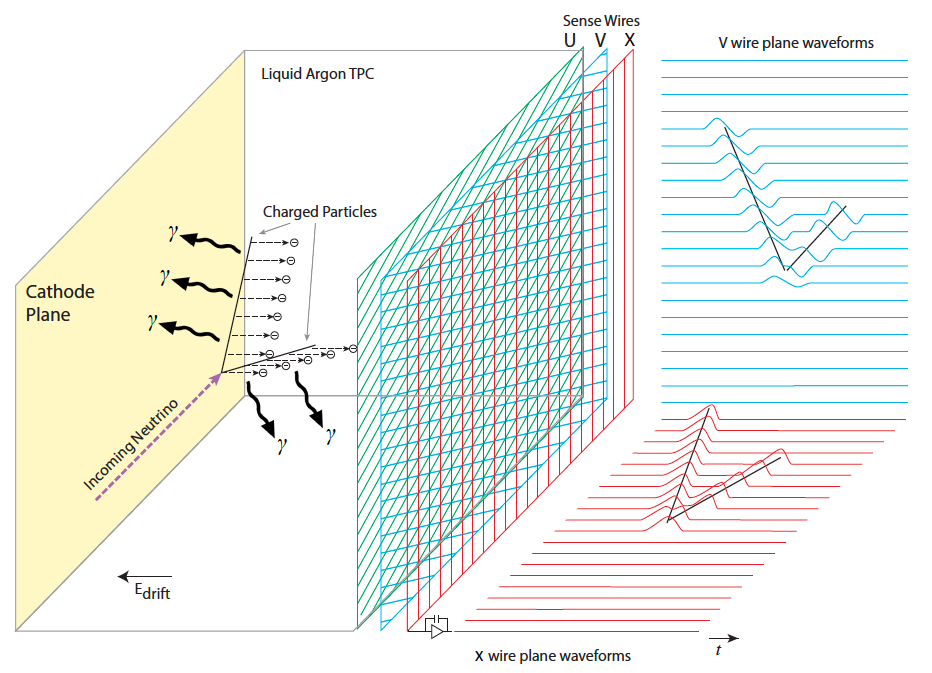
\includegraphics[width=0.8\textwidth]{figures/ch3-DUNE/TheBoPicture.png}
     \caption[Schematic representation of the detection method of liquid argon time projection chambers]{Schematic representation of the detection method of liquid argon time projection chambers \cite{DUNE:2020TDR1}.}
        \label{fig:LArTPCdiagram}
\end{figure}

The liquid argon time projection chamber (LArTPC), first proposed by Carlo Rubbia in 1977 \cite{Rubbia:1977zz}, combines elements of both tracking and scintillator detectors. In a LArTPC, as charged particles travel trough the detector, they produce ionization electrons and prompt vacuum ultra-violet (VUV) scintillation photons. The electrons are drifted by an electric field and collected by a wire plane placed at the anode. The disposition of the wires allows for the reconstruction of a two-dimensional image of the event. The third dimension can be obtained by measuring the drift time of the electrons. The start time is given by the prompt scintillation light, which can be collected by photo-sensors within a few nanoseconds, whereas the drift time is of the order of the microsecond. The basic functioning principles of a LArTPC are illustrated in Fig. \ref{fig:LArTPCdiagram}.

The choice of liquid Argon as a medium is motivated by several key advantages. LAr has a high density, making it a good target for neutrinos. It also exhibits low electron attachment and high electron mobility, allowing for long drift volumes and effective charge transport and collection. Additionally Argon is relatively inexpensive, easy to purify and liquefy and largely chemically inert. LArTPC's are extremely powerful in particle identification, as they produce almost photographic renditions of interaction events, which can be combined with energy loss information. This, for example, allows to distinguish between photon and electron showers, which is extremely valuable in neutrino oscillation experiments. Several detectors using this technology have already taken data (e.g. ICARUS \cite{ICARUS:2004wqc}, MicroBooNE \cite{MicroBooNE:2016pwy}, etc.) and several more are planned for the next generation of neutrino experiments. 
\subsection{Cherenkov detectors}
When a particle travels through a transparent medium faster than the speed of light, it produces a coherent cone of blue light known as Cherenkov radiation. The half angle of the cone $\theta_C$ depends on the refractive index of the medium $n$ and the velocity of the particle $\beta$ as $\cos\theta = 1/n\beta$. The particle travels down the axis of the cone, which makes reconstructing the particle's direction possible.

Two main categories of Cherenkov detectors exist. The first kind consists of densely instrumented artificial tanks such as Super-Kamiokande and SNO. In these detectors either natural or heavy water is contained in a tank lined with photo-multiplier tubes (PMT's). The Cherenkov light produced by electrons or muons is reconstructed as a ring of photons on the PMT's, with significantly different appearances. Muons interact as a single particle producing a long track and they form \enquote{sharp} rings, while electrons initiate electromagnetic showers which form \enquote{fuzzy} rings. As discussed in Sec. \ref{Sec:NuHistory} these detectors have thresholds of the order of 1 MeV and have been heavily used for the study of solar and atmospheric neutrino oscillations. At these energies natural water Cherenkov detectors are mostly sensitive to electron neutrinos, while heavy water detectors are sensitive to all flavours.

The second category of Cherenkov detectors consists of sparsely instrumented neutrino telescopes which include experiments such as IceCube. These detectors make use of very large volumes of natural water which are instrumented with a sparse array of photo-multipliers dispersed through the volume. The thresholds tend to be very high, of the order of tens or hundreds of GeV and the reconstruction of muon tracks tend to be much more efficient than for electronic showers. The cone geometry is not immediately apparent, but can be reconstructed using the time at which each photo-multiplier records a hit. Since the particles that are reconstructed are highly relativistic i.e. $\beta\sim 1$ the aperture of the cone only depends on the refraction index on the material $\cos\theta \sim 1/n$.

\subsection{Nuclear emulsions}
Nuclear emulsions consist of sensitive materials, similar to the ones used for photographic films, which are shaped into slabs and exposed to particle beams. The passage of a charged particle induces chemical changes in the material, which can be used to produce visible tracks once the emulsion is developed. This technique presents several drawbacks: the information that is recorded in the slabs is inherently analogical, cannot be triggered and cannot be accessed in real time, because it requires the development of the photographic material; additionally the slabs cannot be re-used once they have been developed. However, a fine-grained emulsion can provide micrometre accuracy in track positions, making it an ideal choice for reconstructing the decay of extremely short lived particles. For this reason the technique was used  by the DONUT experiment, which is credited with the discovery of the tau-neutrino. 

\section{Passage of particles through matter}
\label{Sec:Passage}
%Get from PDG https://pdg.lbl.gov/2022/reviews/rpp2022-rev-passage-particles-matter.pdf

When a relativistic charged particle moves through a medium, it undergoes electromagnetic interactions with the atomic electrons, leading to energy loss and ionization of the atoms. The energy loss per unit distance traveled $dE/dx$, also known as the stopping power, is described by the Bethe-Bloch formula ~\cite{PDG}. The stopping power varies weakly between materials and only depends on their densities $\rho$. It can thus be written as:
\begin{equation} \label{eq:Bethe}
    -\frac{\textrm{d}E}{\rho\textrm{d}x} = 4\pi N_{A}r_e^2m_ec^2z^2\frac{Z}{A}\frac{1}{\beta^2}\left(\frac{1}{2}\ln{\frac{2m_ec^2\beta^2\gamma^2T_{\textrm{max}}}{I^2}}-\beta^2-\frac{\delta}{2}\right),
\end{equation}
where $N_{A}$ is Avogadro's number, $r_e$ is the classical electron radius, $m_ec^2$ is the electron mass energy, $z$ is the charge of the particle, $Z$ and $A$ are the atomic number and mass of the absorbing material, $\beta$ and $\gamma$ are the usual relativistic factors for the passing particle, $I$ is the material mean excitation energy, $T_{\textrm{max}}$ is the maximum kinetic energy which can be imparted to a free electron in a single collision and $\delta/2$ is a density effect correction factor. The mean energy loss rate for charged particles in different materials is shown in Fig. \ref{fig:Bethe} as a function of the particles velocities $\beta\gamma$ and different particles momenta.

\begin{figure}
    \centering
    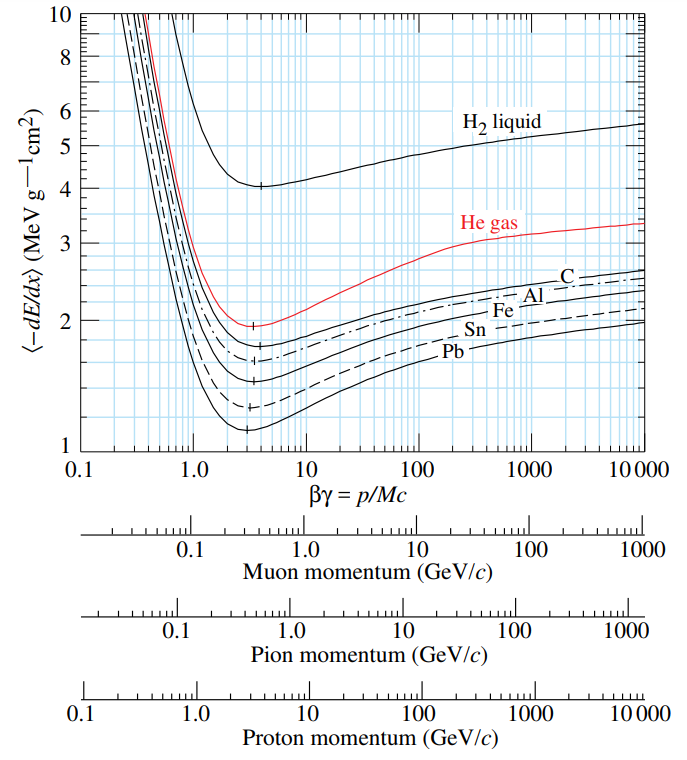
\includegraphics[width=0.7\linewidth]{figures//ch2-Theory/BetheBloch.png}
    \caption[Mean energy loss rate in liquid (bubble chamber) hydrogen, gaseous helium, carbon,aluminum, iron, tin, and lead.]{Mean energy loss rate in liquid (bubble chamber) hydrogen, gaseous helium, carbon,aluminum, iron, tin, and lead. Radiative effects, relevant for muons and pions, are not included. Taken from ~\cite{PDG}. }
    \label{fig:Bethe}
\end{figure}

The stopping power is independent of the mass of the particles and depends on the charge of the incident particle squared $Z^2$. At relatively small velocities $\beta\gamma<3.5$ the $dE/dx$ falls off as $1/\beta^2$. As $\beta$ gets smaller the $\beta^2\gamma^2 = 1/(1-\beta^2)$ term in the logarithm halts the decrease of the stopping power. A minimum is reached at $3 \leq \beta\gamma \leq 4$ at which particle are said to be minimum ionizing particles (MIP's). Beyond the minimum the logarithmic component of the Bethe formula becomes dominant, and the stopping power begins to rise again. This is due to the fact that, as the incident charged particle reaches relativistic energies, its transverse electric field increases, leading to more of the material’s atoms being within range of the particle’s electric field. However, the slope eventually shallows out, due to the fact that  long distance atomic electrons are screened from the electric field of the incident particle by the dielectric effect of the intervening atoms in the material. This phenomenon is known as the \enquote{density effect} and is encapsulated in the $\delta/2$ term in the formula.

From the Bethe-Bloch formula the range $R$ of a charged particle entering a material with an initial energy $E_0$ can be calculated as:
\begin{equation}
    R = \int_{E_0}^{0} \frac{dE}{dE/dx}
\end{equation}
Following the calculation \cite{Frass2009}, the formula gives:
\begin{align}
\label{eq:range}
    R & \propto E_0^{3/2}/\sqrt{m} \\
    R & \propto m(\beta c)^3
\end{align}
From this it follows that, if two particles have the same velocity, the heavier one will travel further, while if they have the same initial kinetic energy, the lighter one will. However, it is important to note that since energy loss is a statistical process, particles starting with the same kinetic energy will produce a spread of different final energies and ranges leading to the phenomenon of range straggling.

A charged particle travelling through a medium will not only lose energy through ionization, but it will also be deflected in its path by a series of small scatters. This behaviour is mostly due to Coulomb scattering from nuclei and is usually referred to as multiple Coulomb scattering or simply multiple scattering (MS). For most small angle scatters the net scattering and displacement distributions are Gaussian in virtue of the central limit theorem. The spread of the distribution of the scattering angle is well defined by the Molière angle which can be calculated using the formula given by Lynch and Dahl~\cite{LYNCH19916}:
\begin{equation}
\label{eq:MoliereAngle}
    \theta_{\textrm{M}} = \frac{13.6 \ \text{MeV}}{\beta pc}z\sqrt{\frac{\Delta d}{X_0}} \left[ 1+0.038\ln{\left(\frac{\Delta d}{X_0 }\frac{z^2}{\beta^2}\right)}\right], 
\end{equation}
where $\Delta d$ is the total distance traveled between two steps and $X_0$ the radiation length in cm.


